\documentclass[pdftex,12pt,fullpage,oneside]{amsart}
\usepackage{hyperref,array,amsmath,psfrag,amssymb,subfigure,tabularx}
\usepackage{multicol}
\usepackage{booktabs}
%\usepackage{vmargin,boxedminipage}
\usepackage[usenames]{color}
\usepackage{datetime}
\usepackage{dcolumn}
\usepackage{wrapfig}
\usepackage{setspace}
\usepackage{url}
\usepackage[english]{babel}
\usepackage{times}
\usepackage{multirow}
\usepackage[pdftex]{graphicx}
\usepackage{lscape}
\usepackage[top=1in,right=1in,left=1in,bottom=1in]{geometry}
\usepackage{array}
\usepackage{booktabs}
\usepackage{hyperref}
\graphicspath{{graphics/}}



%\usepackage[authoryear,sort&compress]{natbib}
\usepackage{natbib}
\bibpunct{(}{)}{;}{a}{}{,}
%\bibdata{/Users/jacobmontgomery/Dissertation/master3}
\bibdata{Flo_Bib_PA}
\begin{document}

\section*{Project Summary}

\thispagestyle{empty}

Testing systematic predictions about future enevts against observed
outcomes is generally seen as the most stringent validity check of
statistical and theoretical models. Yet, political scientists rarely
make predictions about the future.  Empirical models are seldom
applied to out-of-sample data and are even more rarely used to make
predictions about future outcomes. Instead, researchers typically
focus on developing and validating theories that explain past events.

In part, this results from the fact that it is difficult to make
accurate predictions about complex social phenomena. However, research in political science could gain
immensely in its policy relevance if predictions were more common and
more accurate.  Improved forecasting of important political events
would make research more germane to policymakers and the general
public who may be less interested in explaining the past than
anticipating and altering the future.  From a scientific standpoint,
greater attention to forecasting would facilitate stringent validation
of theoretical and statistical models since truly causal models should
perform better in out-of-sample forecasting.

We propose to extend a promising statistical method -- ensemble
Bayesian model averaging (EBMA) -- and to develop software that will
aid researchers across disciplines to make more accurate forecasts.
This project builds on work in the fields of meteorology, fluid
dynamics, and statistics to (1) extend the method for application to a
wider array of outcomes (e.g., binary data), (2) provide freely
available software that implements both maximum likelihood and
Bayesian estimation techniques, and (3) publish papers that provide
accessible explanations of the method and real-world social science
applications.

In essence, EBMA makes more accurate predictions possible by pooling
predictions from multiple forecast models. The weight assigned to each
component is calibrated via its predictive performance in some
training period. These component models can be diverse.These component models can be diverse.  They
need not share covariates, functional forms, or error
structures. Indeed, the components may not even be statistical models,
but may be predictions generated by agent-based models, stochastic
simulations, or subject-matter experts. EBMA pools information from heterogenous
sources to improve forecast accuracy of outcomes determined by complex
processes.  In practice, the method provides superior predictive power
relative to any single component. Further, each component model's
weight can be interpreted as the posterior probability that this
particular model reflects the ``true'' data generating process and
thus facilitates meaningful model comparison.

\subsection*{Intellectual merit:} 
This project will address several substantive questions in political
science with a focus on the field of international relations, where
policymakers have a particular demand for improved forecasting.  We
will also further develop statistical techniques that will improve the
capabilities of researchers across disciplines to produce more
accurate forecasts of future events. The methodological advancement
made in this project will be available to the larger scholarly
community and influence research agendas in multiple fields.  EBMA has
received considerable attention in the fields of statistics,
meteorology, and (to a lesser extent) economics.  Yet, it has not been
advanced in the methodological directions we are proposing here.
Additionally, our work will make EBMA available to a wider
audience of researchers across the physical and social sciences.  This
is particularly important as existing research projects and software
packages are narrowly tailored to the needs of weather forecasting.

\subsection*{Broader impacts:}
The principal investigators are active members of the research
community at the intersection of statistics and the social
sciences. Their work is widely read in political science and other
disciplines. Further, at least two graduate student in political
science will be included in the research and will gain experience in
large-scale research projects.

\newpage
\setcounter{page}{1}

\section*{Project Description}

Testing systematic predictions about future events against observed
outcomes is generally seen as the most stringent validity check of
statistical and theoretical models.  Yet, political scientists rarely
make predictions about the future.  Empirical models are seldom
applied to out-of-sample data and are even more rarely used to make
predictions about future outcomes. Instead, researchers typically
focus on developing and validating theories that explain past events.

In part, this results from the fact that it is difficult to make
accurate predictions about complex social phenomena. However, research in political science could gain
immensely in its policy relevance if predictions were more common and
more accurate.  Improved forecasting of important political events
would make research more germane to policymakers and the general
public who may be less interested in explaining the past than
anticipating and altering the future.  From a scientific standpoint,
greater attention to forecasting would facilitate stringent validation
of theoretical and statistical models since truly causal models should
perform better in out-of-sample forecasting.

We propose to extend a promising statistical method -- ensemble
Bayesian model averaging (EBMA) -- and to develop software that will
aid researchers across disciplines to make more accurate forecasts.
This project builds on work in the fields of meteorology, fluid
dynamics, and statistics to (1) extend the method for application to a
wider array of outcomes (e.g., binary data), (2) provide freely
available software that implements both maximum likelihood and
Bayesian estimation techniques, and (3) publish papers that provide
accessible explanations of the method and real-world social science
applications.

First, we briefly review existing political science research aimed at
forecasting.  We then present the EBMA method.  Next we present
results from empirical applications of the method to the areas of
insurgency events on the Pacific Rim, U.S. presidential elections, and
voting on the U.S. Supreme Court.  We discuss our proposed research
agenda and conclude with a discussion of results from prior NSF
supported research.

\section{Dynamic forecasting in political science}

Although forecasting is a rare exercise in political science, there
are an increasing number of exceptions.  In most cases, ``forecasts''
are conceptualized as an exercise in which the predicted values of a
dependent variable are calculated based on a specific statistical
model and then compared with observed values
\citep[e.g.,][]{Hildebrand:etal:1976}. In many instances, this reduces
to an analysis of residuals.  In others, the focus is on randomly
selecting subsets of the data to be excluded during model development
for cross-validation.  However, there is also a more limited tradition
of making true forecasts about events that have not yet occurred.

An early proponent of using statistical models to make predictions in
the realm of international relations (IR) was Stephen Andriole
\citep{Andriole:Young:1977}. In 1978, a volume edited by Nazli Choucri
and Thomas Robinson \nocite{Choucri:Robinson:1978} provided an
overview of the then current work in forecasting in IR.  Much of this
work was done in the context of policy-oriented research for the
U.S. government during the Vietnam War.  Subsequently, there were a
variety of efforts to create or evaluate forecasts of international
conflict including \citet{Freeman:Job:1979},
\citet{Singer:Wallace:1979}, and \citet{Vincent:1980}. In
addition, a few efforts began to generate forecasts of domestic
conflict \citep[e.g.,][]{Gurr:Lichbach:1986}.  Recent years,
however, have witnessed increasing interest in prediction across a
wide array of contexts in IR.\footnote{An incomplete list of recent
  work would include \citet{Krause:1997}, \citet{Davies:Gurr:1998},
  \citet{Pevehouse:Goldstein:1999}, \citet{Schrodt:Gerner:2000},
  \citet{King:Zeng:2001}, \citet{OBrien:2002}, \citet{BDM:2002},
  \citet{Fearon:Laitin:2003}, \citet{Demarchi:etal:2004}, \citet{Enders:Sandler:2005},
  \citet{Leblang:Satyanath:2006}, \citet{Ward:etal:2007},
  \citet{Brandt:etal:2008}, \citet{Bennett:Stam:2009}, and
  \citet{Gleditsch:Ward:2010}. A summary of classified efforts is
  reported in \citet{Feder:2002}.  An overview of some of the
  historical efforts along with a description of current thinking
  about forecasting and decision-support is given by
  \citet{OBrien:2010}.}  The 2011 special issue of \emph{Conflict
  Management and Peace Science} on prediction in the field of IR
exemplifies this growing emphasis on forecasting
\citep[c.f.,][]{Schneider_etal_2011, Mesquita_2011,
  Brandt_etal_2011}.
  
Outside of IR, forecasting in political science has largely taken
place in the context of election research.  In the 1990s, scholars of
U.S. politics began publishing predictions of presidential elections
\citep{Campbell:1990, Campbell:1992}. These efforts were anticipated
by the efforts of several economists, most notably the forecasts
established by Ray C. Fair (\citeyear{Fair:1978}). As we discuss
below, predicting U.S. presidential and congressional elections has
since developed into a regular exercise.  Moreover, researchers have begun to forecast election outcomes in France
\citep[e.g.,][]{Jerome:1999} and the United Kingdom
\citep[e.g.,][]{Whitely:2005}.\footnote{\citet{Lewis-Beck:2005}
  provides a more in-depth discussion of election forecasting in a
  comparative context.}

While efforts to predict future outcomes remain uncommon, research
that combines multiple forecasts are nearly non-existant.  To our
knowledge, the only non-IR example is the PollyVote project
\citep[c.f.][]{Graefe:2010}, which combines multiple predictions using
simple averages to forecast U.S. presidential elections.

EBMA is a statistical approach that promises to improve prediction of
complex social outcomes and build upon the increased interest in
generating political forecasts.  In essence, EBMA makes more accurate
predictions possible by pooling information from multiple forecast
models. The weight assigned to each component is calibrated via its
predictive performance in some training period. These component models
can be diverse.  They need not share covariates, functional forms, or
error structures. Indeed, the components may not even be statistical
models, but may be predictions generated by agent based models,
stochastic simulations, or subject-matter experts. EBMA pools
information from heterogenous sources to improve forecast accuracy of
outcomes determined by complex processes.

Such ensemble methods have been shown to significantly reduce
prediction error in two important ways.  First, across subject
domains, ensemble predictions are usually more accurate than any
individual component model. Second, they are significantly less likely
to make dramatically incorrect predictions \citep{Armstrong:2001,
  Raftery:2005}.  Combining forecasts not only reduces reliance on
single data sources and methodologies (which lowers the likelihood of
dramatic errors), but also allows for the incorporation of more
information than any one theoretical or statistical model is likely to
include in isolation.  In the next section, we present the details of
the EBMA method that we propose to extend for social science research
with support from the NSF.


\setcounter{section}{1}

\section{Ensemble Bayesian model averaging} 

Predictive models remain underutilized, yet an increasing number of
scholars have developed forecasting models for specific research
domains.  As the number of forecasting efforts proliferate, however,
there is a growing benefit from developing methods to pool across
models and methodologies to generate more accurate forecasts.  Very
often, specific predictive models prove to be correct only for certain
subsets of observations.  Moreover, specific models tend to be more
sensitive to unusual events or particular data issues than ensemble
methods.

The research proposed here will aid the newfound emphasis on
prediction by advancing recent statistical research aimed at
integrating multiple predictions into a single improved forecast.  In particular,
we are adapting an ensemble method first developed for application to
the most mature prediction models in existence -- weather forecasting
models.  To generate predictive distributions of outcomes (e.g.,
temperature), weather researchers apply ensemble methods to forecasts
generated from multiple models \citep{Raftery:2005}.  Thus,
state-of-the-art ensemble forecasts aggregate multiple runs of (often
multiple) weather prediction models into a single unified forecast.

The particular ensemble method we are extending for application to
political outcomes is ensemble Bayesian model averaging (EBMA). First
proposed by \citet{Raftery:2005}, EBMA pools across various forecasts
while meaningfully incorporating \textit{a priori} uncertainty about
the ``best'' model.  It assumes that no particular model or
forecasting method can fully encapsulate the true data-generating
process.  Rather, various research teams or statistical techniques
will reflect different facets of reality. EBMA collects \textit{all}
of the insights from multiple forecasting efforts in a coherent
manner.  The aim is not to choose some ``best'' model, but rather to
incorporate the insights and knowledge implicit in various forecasting
efforts via statistical post-processing. 

EBMA itself is an extension of the Bayesian model averaging (BMA)
methodology \citep[c.f.,][]{Madigan:1994, Draper:1995, Raftery:1995,
  Hoeting:1999, Clyde:2003, Raftery:2003, Clyde:2004} that has
received considerable attention in the field of statistics. BMA was
first introduced to political science by \citet{Bartels:1997} and has
been applied in a number of contexts \citep[e.g.,][]{Bartels:2001,
  Gill:2004, Imai:2004, Geer:2006b}. \citet{Montgomery:2010c} provide a more in-depth discussion of BMA and its applications in
political science.

\subsection{Mathematical intuition}
The basic BMA approach to forecasting is as follows. Assume we have some quantity of interest in the future to forecast,
$\mathbf{y}^*$, based on previously collected training data
$\mathbf{y}^T$ that is fit to $K$ statistical models, $M_1, M_2,
\ldots, M_K$. Each model, $M_k$, is assumed to come from the prior
probability distribution $M_k\sim \pi(M_k)$, and the probability
distribution function (PDF) for the training data is
$p(\mathbf{y}^T|M_k)$. The outcome of interest is distributed
$p(\mathbf{y}^*|M_k$).  Applying Bayes Rule, we get that
\begin{equation} \small
p(M_k|\mathbf{y}^T) = \frac{p(\mathbf{y}^T|M_k)\pi(M_k)}{\underset{k=1}{\overset{K}{\sum}}p(\mathbf{y}^T|M_k)\pi(M_k)}.
\end{equation}
\noindent and the marginal predictive PDF for $y^*$ is
\begin{equation}
\label{BMA-pdf}
\small
p(\mathbf{y}^*) = \underset{k=1}{\overset{K}{\sum}} p(\mathbf{y}^*|M_k)p(M_k|\mathbf{y}^T).
\end{equation}
The BMA PDF (\ref{BMA-pdf}) can be viewed as the weighted average of
the component PDFs where the weights are determined by each model's
performance within the training data.  Likewise, we can simply make a
deterministic estimate using the weighted predictions of the
components, denoted
\begin{equation} \small
E(\mathbf{y}^*) = \underset{k=1}{\overset{K}{\sum}} E(\mathbf{y}^*|M_k)p(M_k|\mathbf{y}^T).
\end{equation}

\subsection{EBMA for dynamic settings}

We now turn to applying this basic BMA technology to prediction in a
dynamic setting.  In generating predictions of important events (e.g.,
domestic crises or international disputes), the task is to first build
a statistical model for some set of observations $S$ in time periods
$T$, which we refer to as the training
period.\footnote{\citet{Sloughter:2007} make predictions for only one
  future time period, and use only a subset of past time-periods (they
  recommend 30) in their training data. Thus, predictions are made
  sequentially with the entire EBMA procedure being re-calculated for
  each future event as observations are moved from the out-of-sample
  period $T^*$ into the training set $T$. Another alternative is to
  simply divide \textit{all} the data into discrete training and test
  periods for the entire procedure.  We use both approaches in our
  examples below.}  Using the same statistical model (or general
technique in the case of subject-expert predictions), we then generate
forecasts, $\mathbf{f}_k$, for observations $S$ in future time periods
$T^*$.

Let us assume, for example, that we have $K$ models forecasting
insurgencies in a set of countries $S$. Each component forecast,
$\mathbf{f}_k$, is associated with a component PDF,
$g_k(\mathbf{y}|\mathbf{f}_k)$, which may be the original predictive
PDF from the forecast model or a bias-corrected forecast.  These
components are the conditional PDFs of outcome $\mathbf{y}$ given the
$k$th forecast, $\mathbf{f}_k$ assuming that $P(M_k | \mathbf{y})
\equiv w_k=1$, or that the posterior odds of model $k$ is unity.

% This
% assumes that $P(M_k | \mathbf{y}) \equiv w_k=1$, or the posterior odds
% of model $k$ is unity.

%  being the ``best''
% forecast in the ensemble. For example, the posterior PDF of an outcome
% $y_{st}$ for some country $s \in S$ in period $t \in T$ given the
% forecast $f_{kst}$ from model $k$ is $g_k(y_{st}|f_{kst})$. 

The EBMA PDF is then a finite mixture of the $K$ component forecasts,
denoted
\begin{equation}
\small
\label{BMA-eq}
p(\mathbf{y}|\mathbf{f}_1, \ldots, \mathbf{f}_K)=\overset{K}{\underset{k=1}{\sum}} w_k
g_k(\mathbf{y}|\mathbf{f}_k),
\end{equation}
\noindent where the weight, $w_k$, is based on forecast $k$'s relative
predictive performance in the training period $T$. The $w_k$'s $\in
[0,1]$ are probabilities and $\sum_{k=1}^Kw_k=1$.  The specific PDF of
for an out-of-sample event, $y_{st^*}$, is therefore
\begin{equation}
\label{BMA-eq2}
\small
p(y_{st^*}|f_{1st^*}, \ldots,
f_{Kst^*})=\overset{K}{\underset{k=1}{\sum}} w_k
g_k(y_{st^*}|f_{kst^*}).
\end{equation}
\subsection{EBMA for normally distributed outcomes}

When forecasting outcomes that are distributed according to the normal
distribution, \citet{Raftery:2005} propose approximating the
conditional PDF as a normal distribution centered at a linear
transformation of the individual forecast, $g_k(\mathbf{y}|\mathbf{f}_k) = N(a_{k0} + a_{k1}\mathbf{f}_k,
\sigma^2)$.  Using \eqref{BMA-eq} above, the EBMA PDF is then
\begin{equation} \small
p(\mathbf{y}|\mathbf{f}_1, \ldots, \mathbf{f}_K) = \overset{K}{\underset{k=1}{\sum}} w_k N(a_{k0} +
a_{k1}\mathbf{f}_k, \sigma^2).
\end{equation}

\subsection{The dichotomous outcome model}

Past work on EBMA does not apply directly to the prediction of many
political events because the assumed PDFs are normal, Poisson, or
gamma. In many settings (e.g., international conflicts), the data are
not sufficiently fine-grained to justify these distributional
assumptions.  Usually, the outcomes of interest are dichotomous
indicators for whether an event (e.g., civil war) has occurred in a
given time period and country. Thus, none of the distributional
assumptions used in past work are appropriate in this context.
Fortunately, it is a straightforward extension of
\citet{Sloughter:2007} and \citet{Sloughter:2010} to deal
appropriately with binary outcomes.\footnote{The method for dealing with
  binary outcomes is implicit in \citet{Sloughter:2007} and
  \citet{Sloughter:2010}, which assume a discrete-continuous %%%% do we want this footnote in the proposal??
  distribution for outcomes that include a logistic component.
  However, they do not explicitly and fully develop the model for
  dichotomous outcomes.  A related strain of research on Dynamic Model
  Averaging \citep[c.f.,][]{Raftery:2010, Muhlbaier:2007} has recently
  been extended for direct application to binary outcomes
  \citep[e.g.,][]{Mccormick:2011, Tomas:2011}.}

We follow \citet{Sloughter:2007} and \citet{Hamill:2004} in using
logistic regression after a power transformation of the forecast to
reduce prediction bias. For notational ease, we assume that $\mathbf{f}_k$ is the
forecast after the adjustment for bias reduction.  Therefore, let
$\mathbf{f}'_k \in [0,1]$ be the forecast on the predicted probability scale
 and
\begin{equation}
\small
%\begin{array}{rl}
\mathbf{f}_k =  \left[(1+\mbox{logit}(\mathbf{f}'_k))^{1/b} - 1\right]I\left[\mathbf{f}'_k>\frac{1}{2}\right]  - \left[(1+\mbox{logit}(|\mathbf{f}'_k|))^{1/b} -  1\right]I\left[\mathbf{f}'_k<\frac{1}{2}\right],
%\end{array}
 \end{equation}
 \noindent where $I[.]$ is the general indicator function.
 \citet{Hamill:2004} recommend setting $b=4$, while
 \citet{Sloughter:2007} use $b=3$.  We found that $b=4$ works best in
 the examples below, but other analysts may try alternative
 specifications. This transformation dampens the effect of extreme observations and reduces over-fitting.

The logistic model for the outcome variables is % \footnote{Likewise, $\mbox{logit } P(\mathbf{y}=0|\mathbf{f}_k) \equiv
 % \mbox{log}\frac{P(\mathbf{y}=0|\mathbf{f}_k)}{P(\mathbf{y}=1|\mathbf{f}_k)}$.}
\begin{equation} \small
\label{one}
\mbox{logit } P(\mathbf{y}=1|\mathbf{f}_k) \equiv \mbox{log}\frac{P(\mathbf{y}=1|\mathbf{f}_k)}{P(\mathbf{y}=0|\mathbf{f}_k)} = a_{k0}+a_{k1}\mathbf{f}_k .
\end{equation}
\noindent The conditional PDF of some within-sample event, given the
forecast $f_{kst}$ and the assumption that $k$ is the true model, can
be written
\begin{equation} 
\label{component-eq}
\small
g_k(y_{st}|f_{kst}) = P(y_{st}=1|f_{kst})I[y_{st}=1]  + P(y_{st}=0|f_{kst})I[y_{st}=0].
\end{equation}
Applying this to \eqref{BMA-eq}, the PDF of the final EBMA model for
$y_{st}$ is
\begin{equation}
\label{pdf}
\small
\begin{array}{rl}
p(y_{st}|f_{1st}, f_{2st}, \ldots, f_{Kst}) = &
\overset{K}{\underset{k=1}{\sum}} w_k [
P(y_{st}=1|f_{kst})I[y_{st}=1] \\
& + P(y_{st}=0|f_{kst})I[y_{st}=0]].\end{array}
\end{equation}

% \begin{equation}
% \label{pdf}
% \small
% \begin{array}{rl}
% p(y_{st}|f_{1st}, f_{2st}, \ldots, f_{Kst}) = &
% \overset{K}{\underset{k=1}{\sum}} w_k [
% P(y_{st}=1|f_{kst})I[y_{st}=1] \\
% & + P(y_{st}=0|f_{kst})I[y_{st}=0]].\end{array}
% \end{equation}

% \begin{equation}
% \label{one}
% \begin{array}{ll}
% \mbox{logit } P(y=1|f_k) & \equiv
% \mbox{log}\frac{P(y=1|f_k)}{P(y=0|f_k)}\\
% & = a_{k0}+a_{k1}f_k .\end{array}
% \end{equation}



% \noindent and

% \begin{equation}
% \label{two}
% \mbox{logit } P(y=0|f_k) \equiv
% \mbox{log}\frac{P(y=0|f_k)}{P(y=1|f_k)}
% \end{equation}



% \begin{equation} 
% \label{component-eq}
% \begin{array}{rl}
% g_k(y_{st}|f_{kst}) = &P(y_{st}=1|f_{kst})I[y_{st}=1]  \\ 
%                     &+ P(y_{st}=0|f_{kst})I[y_{st}=0],
% \end{array}
% \end{equation}

\subsection{Parameter estimation by maximum likelihood and EM
algorithm}

Parameter estimation is conducted using only the data from the
training period $T$.  The parameters $a_{0k}$ and $a_{1k}$ are
specific to each individual component model.  For model $k$, these
parameters can be estimated as traditional linear models where
$\mathbf{y}$ is the dependent variable and the covariate list includes
only $\mathbf{f}_k$ and a constant term.

The difficulty is in estimating the weighting parameters,
$w_k~\forall~ k \in [1, 2, \dots, K]$. One approach we
propose to implement with NSF support is to place priors on all
parameters and conduct a fully Bayesian analysis with Markov chain
Monte Carlo techniques \citep[c.f.][]{Vrugt:2008}.  For the moment,
however, we have followed \citet{Raftery:2005} and
\citet{Sloughter:2007} in using maximum likelihood methods.

With standard independence assumptions, the log-likelihood for the
model weights is
\begin{equation}
\small
  \ell (w_1, \ldots, w_K | a_{01},  \ldots, a_{0K}; a_{11},
  \ldots, a_{1K})= \underset{s,t}{\sum}\mbox{log }p(y_{st} |
  f_{1st}, \ldots, f_{Kst}).
\end{equation}
\noindent where the summation is over values of $s$ and $t$ that index
all observations in the training time period, and $p(y_{st}|f_{1st},
\ldots, f_{Kst}) $ is given by \eqref{pdf}. The log-likelihood
function cannot be maximized analytically, but \citet{Raftery:2005}
and \citet{Sloughter:2007} suggest using the expectation-maximization
(EM) algorithm.  We introduce the unobserved quantities $z_{kst}$,
which represent the posterior probability for model $k$ for
observation $y_{st}$.  The E step involves calculating estimates for
these unobserved quantities using the formula
\begin{equation}
\small
\hat{z}^{(j+1)}_{kst} = \frac{\hat{w}^{(j)}_k
p^{(j)}(y_{st}|f_{kst})}{\overset{K}{\underset{k=1}{\sum}}\hat{w}^{(j)}_kp^{(j)}(y_{st}|f_{kst})},
\end{equation}
\noindent where the superscript $j$ refers to the $j$th iteration of
the EM algorithm.


It follows that $w_k^{(j)}$ is the estimate of $w_k$ in the $j$th
iteration and $p^{(j)}(.)$ is shown in \eqref{pdf}.  Assuming these
estimates of $z_{kst}$ are correct, it is then straightforward to
derive the maximizing value for the model weights. Thus, the M step
estimates these as
$\hat{w}^{(j+1)}_k=\frac{1}{n}\underset{s,t}{\sum}\hat{z}^{(j+1)}_{kst}$,
where $n$ represents the number of observations in the training
dataset.\footnote{In the case of normally distributed data,
  $\hat{\sigma}^{2(j+1)}=\frac{1}{n}\underset{s,t}{\sum}\overset{K}{\underset{k=1}{\sum}}\hat{z}^{(j+1)}_{kst}(y_{st}-f_{kst})^2$.}


The E and M steps are iterated until the improvement in the
log-likelihood is no larger than some pre-defined
tolerance.\footnote{Although the log-likelihood will increase after each
  iteration of the algorithm, convergence is only guaranteed to a
  local maximum of the likelihood function.  Convergence to the global
  maximum is not assured, and the model may be sensitive to initial
  conditions. In future research, we will explore these convergence
  issues more fully with special attention paid to comparison with
  fully Bayesian implementations. In the examples below, we begin with
  the assumption that all models are equally likely, $w_k =
  \frac{1}{K} ~ \forall ~ k \in [1, \ldots, K]$.}



\subsection{Ensemble prediction}

With these parameter estimates, it is now possible to generate
ensemble forecasts. If our forecasts, $\mathbf{f}_k$, are generated
from a statistical model, we now generate a new prediction,
$f_{kst^\ast}$, from the previously fitted models. For convenience,
let $\hat{\mathbf{a}}_k \equiv (\hat{a}_{k0}, \hat{a}_{k1})$. For some
dichotomous observation in country $s\in S$ in the out-of-sample
period $t^\ast\in T^\ast$, we can see that
\begin{equation}
\label{nothing}
{\small
P(y_{st^*} = 1 | f_{1st^\ast}, \ldots, f_{Kst^\ast} ;  \hat{\mathbf{a}}_1,
 \ldots, \hat{\mathbf{a}}_K ; \hat{w}_1, \ldots, \hat{w}_K) =
 \overset{K}{\underset{k=1}{\sum}} \hat{w}_k
 \mbox{logit}^{-1}\left(\hat{a}_{k0} +  \hat{a}_{k1}f_{kst^\ast}\right).}
\end{equation}



\section{Empirical applications}

\subsection{Application to insurgency forecasting}

Our first example applies the EBMA method to data
collected for the Integrated Crisis Early Warning Systems (ICEWS)
project sponsored by the Defense Advanced Research Projects Agency
(DARPA).  The task of the ICEWS project is train models on data
(focusing on five outcomes of interest) for 29 countries for every month from 1997
through the present and to then make accurate predictions about
expected crisis events over the subsequent three months.\footnote{The
  twenty-nine countries are Australia, Bangladesh, Bhutan, Cambodia,
  China, Comoros, Fiji, India, Indonesia, Japan, Laos, Madagascar,
  Malaysia, Mauritius, Mongolia, Myanmar, Nepal, New Zealand, North
  Korea, Papua New Guinea, Philippines, Russia, Singapore, Solomon
  Islands, South Korea, Sri Lanka, Taiwan, Thailand, and Vietnam. This
  set is not a random sample, but rather constitutes the countries of
  population greater than $500,000$ that are in the area of
  responsibility of the US Pacific Command.}  For purposes of
demonstration, we focus on only one of these outcomes -- violent
insurgency.


%  The
% countries in PACOM include about $50\%$ of the total world population,
% along with five of the largest military powers (China, Russia, India,
% North \& South Korea). The countries range from democratic to
% authoritarian, from tiny to enormous, from landlocked to archipelago,
% and vary widely on almost any social or economic indicator you might
% imagine. One of the main missions of the U.S. Pacific Command is to
% enhance stability in the Asia-Pacific region by promoting security,
% cooperation, encouraging peaceful development. As such it is
% interested in the ebb and flow of events in this region.

The bulk of the data for the ICEWS project is gleaned from natural
language processing of a continuously updated harvest of news stories
(primarily taken from Lexus/Nexus and Factiva archives). These are
digested with a version of the TABARI processor for events developed
by Philip Schrodt and colleagues in the context of the Event Data
Project (see \url{http://eventdata.psu.edu/} for more details).  These
data are augmented with a variety of covariates including:
country-level attributes (coded on a monthly or yearly basis) from the
Polity and World Bank datasets, information about election cycles (if
any), events in neighboring countries, and the length of shared
borders with neighboring countries.

\subsubsection{Component Models}

In the remainder of this subsection, we apply EBMA to make predictions
for the occurrence of insurgency in these 29 countries.  We estimate
three exemplar statistical models using data for the in-sample period
ranging from January 1999 to December 2008 and fit an EBMA model.  We
then make out-of-sample forecasts for the period from January 2009 to
December 2010 for the component and EBMA models.  To provide variation
in the complexity (as well as accuracy) of the components, we included
the following models.

\begin{list}{\labelitemi}{\leftmargin=1em}
\item \textbf{SAE}: This is one model developed as part of the ICEWS
  project and was designed by Strategic Analysis Enterprises. It is
  specified as a simple generalized linear logistic model including 27 different
  independent variables.\footnote{See
    \url{strategicanalysisenterprises.com} for more details.  All data
    and models will be included in a replication dataset at the time
    of publication.}  All of the variables are taken from the ICEWS
  event-stream data.
\item \textbf{GLM}: For the purposes of demonstrating the properties
  of the EBMA method, we estimated a crude logistic model that
  includes only \textit{population size} and \textit{GDP growth} (both
  lagged three months).
\item \textbf{LMER}: This is a generalized linear mixed effects model
  using a logistic link function and including random country-level
  intercepts. In addition to the variables from the GLM model, the
  list of covariates includes: the \textit{executive constraint} and
  \textit{competitiveness of participation} variables from the Polity
  IV dataset \citep{PolityIV}, \textit{proximity to
    election},\footnote{This is calculated as the number of days to the
    next or from the last election, whichever is closer.} and a
  \textit{spatial lag} that reflects recent occurrences of
  insurgencies in the countries' geographic
  neighbors.\footnote{Geographical proximity is measured in terms of the
    length of the shared border between the two countries.}
\end{list}

\subsubsection{Results}

Table \ref{InSam1} shows the EBMA model parameters as well as fit
statistics associated with the individual component models and the
EBMA predictions for the in-sample time period. The first column shows
the weights that the EBMA model assigned to each component. As can be
seen, the GLM model is effectively excluded, while the SAE model
carries the greatest weight followed by the LMER model.  The constant
term associated with each component corresponds to the term $a_{k0}$
in (\ref{one}), while the predictor corresponds to $a_{k1}$.
The other columns in Table \ref{InSam1} are fit statistics.  AUC is
the area under the Receiver-Operating Characteristic (ROC) curve. The
advantage of using ROC curves is that it evaluates forecasts in a way
that is less dependent on an arbitrary cutoff point.  A value of 1
would mean that all observations were predicted correctly at all
possible cutoff points \citep{King:Zeng:2001}.


\begin{table}[h!]
\small
% latex table generated in R 2.12.0 by xtable 1.5-6 package
% Thu May 12 10:47:15 2011
\begin{center}
  \caption{\footnotesize In-sample results: Estimated model weights,
    parameters, and fit statistics for EBMA deterministic forecast and
    all component forecasts of insurgency in 29 countries of the
    Pacific rim.}\label{InSam1}
\begin{tabular}{l rrrrrrrrr}
  \toprule
 & Weight & Constant & Predictor & AUC & PRE & Brier & \% Correct \\ 
  \midrule
  SAE & 0.57 & 0.04 & 7.46 & 0.96 & 0.48 & 0.04 & 94.11\\ 
  LMER & 0.43 & 6.08 & 28.25 & 0.96 & 0.01 & 0.07 & 88.79\\ 
  GLM & 0.00 & 0.57 & 8.16 & 0.65 & 0.00 & 0.10 & 88.65\\ 
  EBMA &  &  &  & 0.97 & 0.55 & 0.04 & 94.94\\ 
   \bottomrule
n=3,480\\
\end{tabular}
\end{center}
\end{table}


\begin{wrapfigure}{L}{.6\textwidth}
\caption{\footnotesize Separation plots for in-sample predictions of the ICEWS data (n=3,480).  For each model,
  observations are shown from left to right in order of increasing
  predicted probability of insurgency (shown as the black line).  Observations where
insurgency actually occurred are shown in red.}
\label{InSam1sep}
\begin{center}
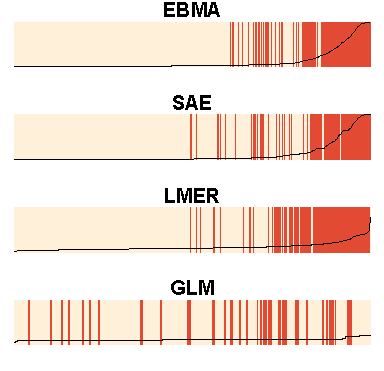
\includegraphics[]{Insamplenew.pdf}
\end{center}
\end{wrapfigure}

We compare the models using three additional metrics.  The
proportional reduction in error (PRE) is the percentage increase of
correctly predicted observations relative to some pre-defined base
model. In this case, the base model is predicting ``no insurgencies''
for all observations.  Insurgencies are relatively rare events.  Thus,
predicting a zero for all observations leads to an 89\% correct
prediction rate. The Brier score is the average squared deviation of
the predicted probability from the true event (0 or 1).  Thus, a lower
score corresponds to higher forecast accuracy \citep{Brier:1950}.
Finally, we calculate the percentage of observations that each model
would predict correctly using a 0.5 threshold on the predicted
probability scale.

There are two aspects of Table \ref{InSam1} that are important to
note.  First, the EBMA model does at least as well (and usually
better) than all of the component models on each our model fit
statistics.  The EBMA model has the highest AUC, PRE, and \% correct.
In addition, it is tied for the lowest Brier score with the SAE model.
Second, in this example the EBMA procedure assigns probability weights
to each model according to their in-sample performance.  The largest
model weight (0.57) is assigned to the SAE model, which appears to be
the best (or tied for the best) component as measured by all of our
fit statistics. Meanwhile, the smallest weight (0.00) is assigned to
the rudimentary GLM model.



% % latex table generated in R 2.11.1 by xtable 1.5-6 package
% % Sat Mar  5 17:06:38 2011
% \begin{table}[ht]
% \begin{center}
% \caption{model statistics -- in-sample predictions}\label{InSam1}\begin{tabular}{rrrrrrrr}
%   \hline
% & Weight & Constant & Predictor & AUC & PRE & Brier & \% Correct
% \\
%   \hline
% Lmer Politics & 0.48 & 0.19 & 7.88 & 0.97 & 0.41 & 0.04 & 93.28
% \\
%   Glm 1 & 0.00 & 0.61 & 8.32 & 0.61 & 0.00 & 0.10 & 88.65 \\ 
% Lmer Politics 2 & 0.15 & 6.08 & 28.25 & 0.96 & 0.01 & 0.07 &
% 88.79 \\
%   Glm 2 & 0.00 & 0.57 & 8.16 & 0.65 & 0.00 & 0.10 & 88.65 \\ 
%   Lmer 3 & 0.01 & 4.56 & 23.41 & 0.93 & 0.01 & 0.07 & 88.74 \\ 
%   SAE & 0.36 & 0.04 & 7.46 & 0.96 & 0.48 & 0.04 & 94.11 \\ 
%   BMA &  &  &  & 0.98 & 0.48 & 0.04 & 94.11 \\ 
%    \hline
% \end{tabular}
% \end{center}
% \end{table}

Figure \ref{InSam1sep} shows separation plots for the EBMA model and
the individual components \citep{Greenhill:2011}. In each plot, the
observations are ordered from left to right by increasing predicted
probabilities of insurgency (as predicted by the particular
model). The black line corresponds to the predicted probability
produced by the relevant model for each observation and actual
occurrences of insurgencies are colored red.  Figure \ref{InSam1sep}
shows visually that the GLM model performs very poorly, whereas of the
SAE model is the best component.  More importantly, the overall best
performance is associated with the EBMA forecast. The separation plots
show that the EBMA model produces few false positives and even fewer
false negatives than any of the component models.




% latex table generated in R 2.12.0 by xtable 1.5-6 package
% Thu May 12 10:46:44 2011
%\begin{wraptable}{R}{.5\textwidth}
\begin{table}
\small
\begin{center}
\caption{\footnotesize Out-of-sample results: Fit statistics for EBMA
    deterministic forecast and all component model forecasts of
    insurgency in 29 countries of the Pacific rim.}\label{OutSam1}
\begin{tabular}{l rrrrrrr}
  \toprule
 & AUC & PRE & Brier & \% Correct \\ 
  \midrule
  SAE &  0.96 & 0.04 & 0.06 & 89.80 \\ 
  LMER & 0.97 & 0.00 & 0.07 & 89.37\\ 
  GLM & 0.84 & 0.00 & 0.09 & 89.37\\ 
  EBMA & 0.96 & 0.18 & 0.05 & 91.24 \\ 
   \bottomrule
n=696 \\
\end{tabular}
\end{center}
\end{table}



The more interesting evaluation of the EBMA method is its
out-of-sample predictive power. Table \ref{OutSam1} shows fit
statistics for the individual components as well as the EBMA forecasts
for observations in the 24 months following the training period.
While the EBMA model has a marginally smaller area under the ROC curve
than the LMER models, it outperforms all component models on the other
metrics. In particular, the EBMA model has the highest PRE at 0.18.
Since it is possible to predict 89.22\% of these observations
correctly by forecasting no insurgency, an 18\% reduction of error
relative to the baseline model is quite substantial.




% % latex table generated in R 2.11.1 by xtable 1.5-6 package
% % Sun Mar  6 14:07:32 2011
% \begin{table}[ht]
% \begin{center}
% \caption{model statistics -- out-of-sample
% predictions}\label{OutSam1}
% \begin{tabular}{rrrrr}
%   \hline
% & AUC & PRE & Brier & \% Correct \\ 
%   \hline
% Lmer Politics & 0.94 & 0.05 & 0.06 & 89.94 \\ 
%   Glm 1& 0.72 & 0.00 & 0.09 & 89.37 \\ 
%   Lmer Politics 2  & 0.97 & 0.00 & 0.07 & 89.37 \\ 
%   Glm 2 & 0.84 & 0.00 & 0.09 & 89.37 \\ 
%   Lmer 3 & 0.97 & 0.00 & 0.07 & 89.37 \\ 
%   SAE & 0.96 & 0.04 & 0.06 & 89.80 \\ 
%   BMA & 0.96 & 0.11 & 0.05 & 90.52 \\ 
%    \hline
% \end{tabular}
% \end{center}
% \end{table}

Figure \ref{OutSam1sep} shows the separation plots for the components
as well as the EBMA forecasts for the out-of-sample data.  The EBMA
model performs better than any of the individual components, with high
predicted probabilities for most observed insurgencies.  Taking
both the fit statistics and the visual evidence together, we can
conclude that the EBMA model leads to a substantial improvement in
out-of-sample forecasts relative to its components.



\begin{wrapfigure}{L}{0.6\textwidth}
\caption{\footnotesize Separation plots for out-of-sample predictions of the ICEWS
  data (n=696).  For each model,
  observations are shown from left to right in order of increasing
  predicted probability (shown as the black line).  Observations where
insurgency actually occurred are shown in red.}
\label{OutSam1sep}
\begin{center}
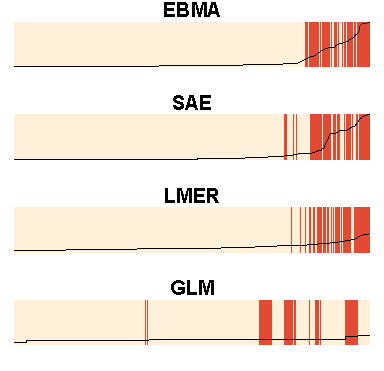
\includegraphics[]{OutSampleNew.pdf}
\end{center}
\end{wrapfigure}



\subsection{Application to US presidential election forecasts}
For the past several U.S. election cycles, a number of research teams
have developed forecasting models and published their predictions in
advance of Election Day.  For example, before the 2008 election, a
symposium of forecasts was published in \emph{PS: Political Science
  and Politics} with forecasts of presidential and congressional vote
shares developed by \citet{Campbell:2008}, \citet{Norpoth:2008},
\citet{Lewis-Beck:Tien:2008}, \citet{Abramowitz:2008},
\citet{Erikson:Wlezien:2008}, \citet{Holbrook:2008},
\citet{Lockerbie:2008} and \citet{Cuzan:Bundrick:2008}.  Responses to
the forecast were published in a subsequent issue. Earlier, in 1999,
an entire issue of the \textit{International Journal of Forecasting}
was dedicated to the task of predicting presidential elections
\citep{Brown:1999}.  Predicting presidential elections has also drawn
the attention of economists seeking to understand the relationship
between economic fundamentals and political outcomes.  Two prominent
examples include work by Ray Fair (\citeyear{Fair:2010}) and Douglas
Hibbs (\citeyear{Hibbs:2000}).

\subsubsection{Component Models}

In the rest of this subsection, we replicate several of these models and
demonstrate the usefulness of the EBMA methodology for improving the
prediction of single important events.  We include six of the most widely cited
presidential forecasting models.
\begin{list}{\labelitemi}{\leftmargin=1em}
\item \textbf{Campbell}: Campbell's ``Trial-Heat and Economy Model''
  \citep{Campbell:2008}
\item \textbf{Lewis-Beck/Tien}: Lewis-Beck and Tien's ``Jobs Model Forecast'' \citep{Lewis-Beck:Tien:2008}
\item \textbf{Erikson/Wlezien}: Erikson and Wlezien's ``Leading Economic Indicators
  and Poll'' forecast\footnote{We replicated Column 2 in Table 2 from \citet{Erikson:Wlezien:2008}.}
\item \textbf{Fair}: Fair's presidential vote-share model\footnote{The model here replicates Equation 1 in \citet{Fair:2010}.}
\item \textbf{Hibbs}: Hibbs' ``Bread and Peace Model'' \citep{Hibbs:2000}
\item \textbf{Abramowitz}: The ``Time-for-Change Model'' created by
  \citet{Abramowitz:2008}
\end{list}
\noindent With the exception of the Hibbs forecast, the models are
simple linear regressions. The dependent variable is the share of the
two-party vote received by the incumbent-party candidate.\footnote{The
  data to replicate the models by \citet{Abramowitz:2008},
  \citet{Campbell:2008}, \citet{Erikson:Wlezien:2008}, and
  \citet{Lewis-Beck:Tien:2008} were provided in personal
  correspondence with the respective authors.  The remaining data were
  downloaded from the web sites of Ray C. Fair \nocite{Fair2011} and
  Douglas Hibbs \nocite{Hibbs2011}.}


\subsubsection{Results}

Rather than selecting a single training period (as in the insurgency
analysis) we generate sequential predictions.  For each year from 1976
to 2008, we use all available prior data to fit the component
models.\footnote{For example, the Fair model uses data for election
  results beginning in 1916 while the Abramowitz model begins with
  data from the 1952 election. }  We then fit the EBMA model using the
components' in-sample performances for election years beginning with
1952 (the year when all models begin generating predictions).  For
example, to generate predictions for the 1988 election, we used the
in-sample performance of each component for the 1952-1984 period to
estimate model weights.\footnote{Results in this section were computed
  using modifications of the `ensembleBMA' package
  \citep{Fraley:2010b, Fraley:Forthcoming}.  Because of the paucity of
  data, we did not apply any bias correction to these forecasts.  Thus,
  the predictor and constant, denoted $a_{0k}$ and $a_{1k}$ above, are
  constrained to zero and one respectively.}

Table \ref{Pres-Year-Res} provides exemplar results for the 2004 and 2008
elections.  Table \ref{Pres-Year-Res} shows the
weights assigned to each model as well as the in-sample root mean
squared error (RMSE) and mean absolute error (MAE) for the components
and the EBMA forecasts.   The table also shows the out-of-sample prediction
errors, calculated as $y_{predicted}-y_{observed}$, for each component
model and the EBMA forecast. 

\begin{table}[ht!]
  \caption{\footnotesize Prediction errors, model weights, and in-sample fit
    statistics for component and EBMA forecasts of the 2004 and 2008
    elections.  Models are sequentially fit using all prior elections.
    The EBMA model does better than all components on in-sample fit
    statistics.  Although it does not necessarily make the most accurate
    prediction for any given year, it is less likely to make
    dramatic forecasting errors.}
\label{Pres-Year-Res} \small
\begin{center}
\begin{tabular}{l rrrrrrrr}	
  \toprule
   &\multicolumn{4}{c}{\textit{2004 Election}} &\multicolumn{4}{c}{\textit{2008 Election}} \\ 
 &	Weights&	RMSE &MAE &\shortstack{Pred. \\ Error}
 &Weights&	RMSE&	MAE &  \shortstack{Pred.\\  Error}\\
\midrule
 Campbell               &0.40&1.71&1.33 &0.53&0.36&1.65&1.28&6.33\\
  Lewis-Beck/Tien 	&0.00&1.67&1.42&$-$0.41&	0.17&1.61&1.33&$-$2.65\\
  Erikson/Wlezien 	&0.00&2.67&2.06&4.76&0.17&2.81&2.18&$-$0.14\\
  Fair                      	&0.48&2.07&1.47&4.82&0.00&2.22&1.80&$-$2.02 \\
  Hibbs                   	&0.12&1.95&1.38&1.54&0.25&1.92&1.38&$-$1.39\\
  Abramowitz        	&0.00&1.50&1.18&2.20&0.06&1.53&1.26&$-$2.37\\
  EBMA                    	&	       	&1.29&1.01&2.08&
  &1.30&1.01&$-$0.53\\
\bottomrule
\end{tabular}
 \end{center}
 \end{table}


The example results in Table \ref{Pres-Year-Res} illustrate three
important points.  First, the EBMA model again does better than any
individual component on in-sample measures of model fit (i.e., RMSE
and MAE).  Second, these results demonstrate that EBMA is not
guaranteed to generate the most accurate prediction for any single
observation.  Thus, in each year some component models come closer to
predicting the actual outcome.  However, the EBMA forecasts will very
rarely provide egregiously wrong predictions (e.g., the Campbell model
in 2008 and the Fair model in 2004) since it borrows predictions from
multiple components.  Moreover, as we show below, in the aggregate the
EBMA model tends to provide the best forecast over time.

Third, Table \ref{Pres-Year-Res} shows it is clear that there is
not as clean a relationship between in-sample model performance and
model weights as in the insurgency example.  For instance, the weight
for the Abramowitz model in 2008 is 0.06 even though it has the lowest
RMSE and MAE of any component.  The diminished relationship between
in-sample performance and weight is a result of high in-sample
correlations between forecasts.
%\note{The correlation matrix between
  %fitted-values of the model for the
  %1952-2008 period is: \\
%\begin{tabular}{l  rrrrrr}
  %\toprule
 %& \textbf{C}& \textbf{L} & \textbf{E}& \textbf{F} & \textbf{H} & \textbf{A} \\ 
  %\midrule
%\textbf{C}ampbell& 1.00 & & & & & \\ 
 %\textbf{L}ewis-Beck/Tien& 0.93 & 1.00 & & & & \\ 
%\textbf{E}rikson/Wlezien & 0.85 & 0.86 & 1.00 & & & \\ 
%\textbf{F}air & 0.87 & 0.88 & 0.91 & 1.00 & & \\ 
%\textbf{H}ibbs& 0.91 & 0.91 & 0.87 & 0.89 & 1.00 & \\ 
%\textbf{A}bramowitz & 0.94 & 0.96 & 0.90 & 0.90 & 0.93 & 1.00 \\ 
 %  \bottomrule
% \end{tabular}.}  For
%instance, fitted values for the Abramowitz model are correlated at
%0.94 with the Campbell model and at 0.96 with the Lewis-Beck/Tien
%model. Thus, conditioned on knowing these forecasts, the Abramowitz
%component provides limited additional information.  


% \begin{figure}[ht!]
%   \caption{\footnotesize Weighted predictive PDF's for component
%     models (colored lines) and the full EBMA predictive PDF (thick
%     black line).  The ``O'' shows the deterministic EBMA prediction
%     and the ``X'' shows the actual observed value for the given year.
%     The dashed line is the 95\% credible interval for the EBMA
%     predictive PDF.}
% \label{PresPlots}
% \begin{center}
% 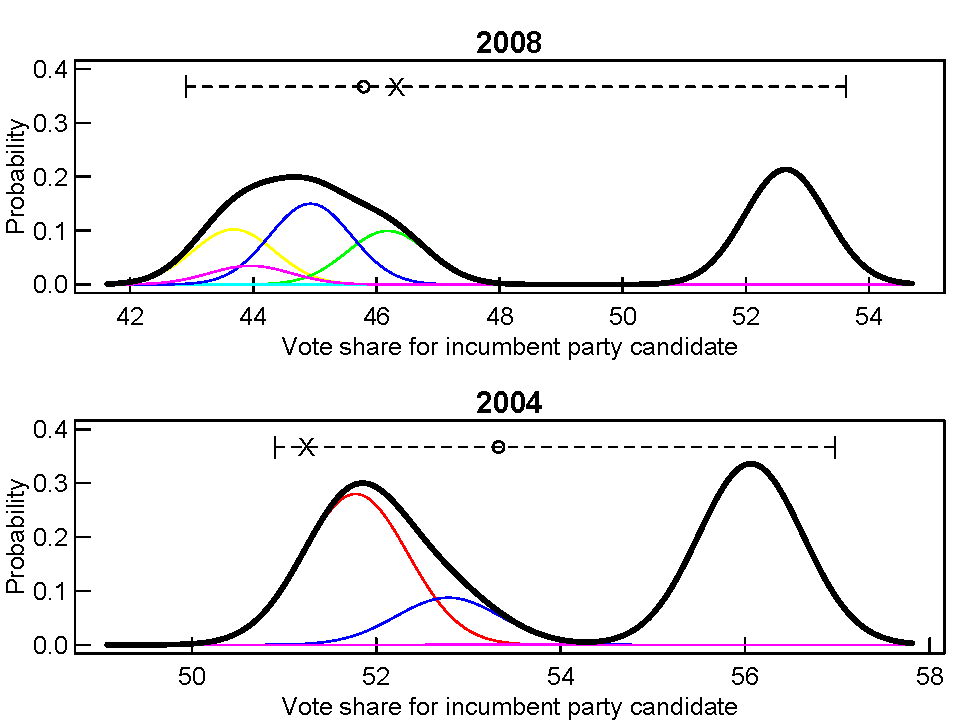
\includegraphics[width=5 in]{PresPlots.PDF}
% \end{center}
% \end{figure}

With the 2004 and 2008 examples in mind, we now turn to the relative
out-of-sample performance of the EBMA and component forecasts across
the entire 1976-2008 period.  Table \ref{Pres-Res} shows the
out-of-sample RMSE and
MAE statistics as well as the percentage of observations that fall
within the 67\% and 95\% predictive intervals for each.  For our
purposes here, the main result in Table \ref{Pres-Res} is that the
EBMA model again outperforms all components.  The first two columns
show this to be true in terms of predicted error (RMSE and MAE).


\begin{table}[ht!]
  \caption{\footnotesize Fit statistics and observed coverage
    probabilities for sequentially generated out-of-sample predictions of
    presidential elections from 1976-2008.  EBMA outperforms its
    component models on all metrics.}
\label{Pres-Res} \small
\begin{center}
\begin{tabular}{lrrrrr}
\toprule
                        &              &              & \multicolumn{2}{c}{Coverage} \\ 
                    	&	RMSE&	MAE	&67\% &   90\%      \\
\midrule
EBMA	           &	1.72	&	1.47	&	0.67	&	0.89	\\
Campbell	           &	2.74	&	1.99	&	0.67	&	0.78	\\
Lewis-Beck/Tien&	2.27	&	1.82	&	0.89	&	1.00	\\
Erikson/Wlezien&	2.88	&	2.16	&	0.78	&	1.00	\\
Fair	                   &	4.01	&	3.20	&	0.44	&	0.78	\\
Hibbs	           &	2.81	&	2.24	&	0.44&      0.78 \\
Abramowitz	   &	2.27	&	2.05	&	0.33	&     0.78	\\

\bottomrule
\end{tabular}
\end{center}
\end{table}

 In addition, the coverage statistics demonstrate better calibration
 of EBMA forecasts relative to its component models.  For instance,
 the observed outcome falls within the 67\% predictive interval for
 the Abramowitz model only three out of nine times, while it covers the
 observed values eight out of nine times for the Lewis-Beck/Tien
 model.  Meanwhile, the EBMA 90\% an 67\% predictive intervals are
 nearly perfectly calibrated.

 In a well-calibrated forecasting model, out-of-sample outcomes should
 fall within predictive intervals at a rate corresponding to their
 size.  For instance, the goal is for two-thirds of all out-of-sample
 observations to fall within of their respective 67\% predictive
 intervals.  Poorly calibrated models will tend to be produce
 predictive intervals that are either too narrow, generating
 inaccurate predictions, or too large, generating predictions that are
 accurate but too vague to be useful. For example, two of the most  % this is where the large figure was, do we want that in here,  
 accurate forecasts, the Lewis-Beck/Tien and Erikson/Wlezien models,  % maybe needs some editing
 make very imprecise predictions.  Thus, although they have very good
 coverage, it is at least partly because their estimates are so
 inexact.  The Campbell, Abramowitz, and Hibbs models provide more
 reasonable predictive intervals, but are less accurate than
 EBMA. Meanwhile, the Fair model falls somewhere in between these two
 groupings.	


 Finally, it is worth noting an example -- very noticeable in this
 data -- of the kinds of problems that may arise when relying on a
 single model for making predictions.  From 1952 to 2004, the Campbell
 model was consistently one of the strongest performers.  Indeed, it
 made the most accurate forecast of the 2004 election.  However, one
 of the crucial variables in this model comes from polling data
 measured in early September.  As a result of the particularly late
 timing of the Republican Convention in 2008, it was the only model to
 forecast a victory for John McCain.  By relying on a wider array of
 data sources and methodologies, EBMA reduces the likelihood of such
 large misses without completely eliminating the general insights
 captured by individual models that may on occasion be wide of the
 mark.

% There should probably be some moving conclusion to this section, but
% I don't know what it should be.  

\subsection{Application to Supreme Court Forecasting Project}

Our final application of EBMA is a re-analysis of data from the
Supreme Court Forecasting Project \citep{Ruger:2004,
  Martin:2004}.\footnote{Additional details about the project,
  replication files, as well as a complete listing of cases and expert
  forecasts are available at: \url{http://wusct.wustl.edu/index.php}.}
This example highlights the ability of EBMA to handle forecasts
generated by classification trees, subject experts, and other sources.

Throughout 2002-2003, a research team consisting of Andrew
Martin, Kevin Quinn, Theodore Ruger, and Pauline Kim (henceforward
MQRK) generated two sets of forecasts for every pending case.  First,
using data about case characteristics and justices' past voting
patterns, MQRK developed classification trees to generate a binary
forecasts for the expected vote of each justice on each case (voting
to affirm the lower court opinion is coded as a 1).  Second, MQRK
recruited a team of 83 legal experts to make forecasts on particular
cases in their specialty area.  The list included academics, appellate
attorneys, former Supreme Court clerks, and law school deans.  MQRK
attempted to recruit three expert forecasts for each case, although
this was not possible for all cases.

The statistical model makes predictions for all 67 cases included in
the MQRK analysis.  Thus, we include the binary model predictions as
one component forecast. However, the individual legal experts made
predictions on only a handful of cases. Owing to the paucity of the
data for each judge, we pooled them together and treat all of the
expert opinions as part of a single forecasting effort.  We coded the
expert forecast to be the mean expert prediction. This implies that
the expert forecast predicts a vote to affirm if a majority of experts
polled for that case predict an affirming vote.  We fit an EBMA model
using all cases with docket numbers dating from 2001 (n=395).\footnote{The
  in-sample results are available upon request.} and made EBMA forecasts for
the remaining 296 cases with 2002 docket numbers.

 \subsubsection{Results}

Table \ref{SC-Res} shows the component weights for the two forecasts
and the out-of-sample fit statistics for the MQRK classification
trees, subject experts, and EBMA forecasts. Once again, the results
show that the EBMA procedure outperforms all components (even when
there are only two).  In terms of AUC, Brier scores, and correct
predictions, the EBMA forecast outperforms both the statistical model
and the combined subject experts.  In addition, EBMA scores
substantially better on the PRE metric.\footnote{The baseline model here
  is prediction that all votes will be to reverse the lower court.
  This baseline model is correct for roughly 70\% of the votes in the
  out-of-sample period.}

% latex table generated in R 2.12.0 by xtable 1.5-6 package
% Thu May 12 17:11:59 2011
\begin{table}[ht]
  \caption{\footnotesize Out-of-sample results for U.S. Supreme Court
    example.  The table shows fit statistics for the EBMA deterministic
    forecast and component forecasts of U.S. Supreme Court votes on
    cases in the 2002-2003 session with 2002 docket numbers.   EBMA
    outperforms its component models on all metrics. }
\label{SC-Res} \small
\begin{center}
\begin{tabular}{lrrrrrrr}
\toprule
 & Weight & AUC & PRE & Brier & \% Correct   \\ 
\midrule
MQRK model& 0.32  & 0.66 & -0.02 & 0.29 & 70.56   \\ 
Subject experts & 0.68 & 0.62 & 0.15 & 0.23 & 75.23  \\ 
EBMA forecast&  & 0.70 & 0.21 & 0.18 & 77.10  \\ 
\bottomrule
n=214 
\end{tabular}
\end{center}
\end{table}


%\begin{figure}[ht!]
%\caption{\footnotesize Separation plots for out-of-sample predictions
%  of the Suprem Court votes (n=214). For each model, observations are
 % shown from left to right in order of increasing predicted
 % probability (shown as the black line).  Instances where justices voted
  %to affirm the lower court opinion (coded as 1) are colored in red.}
%\label{SCPLOT}
%\begin{center}
%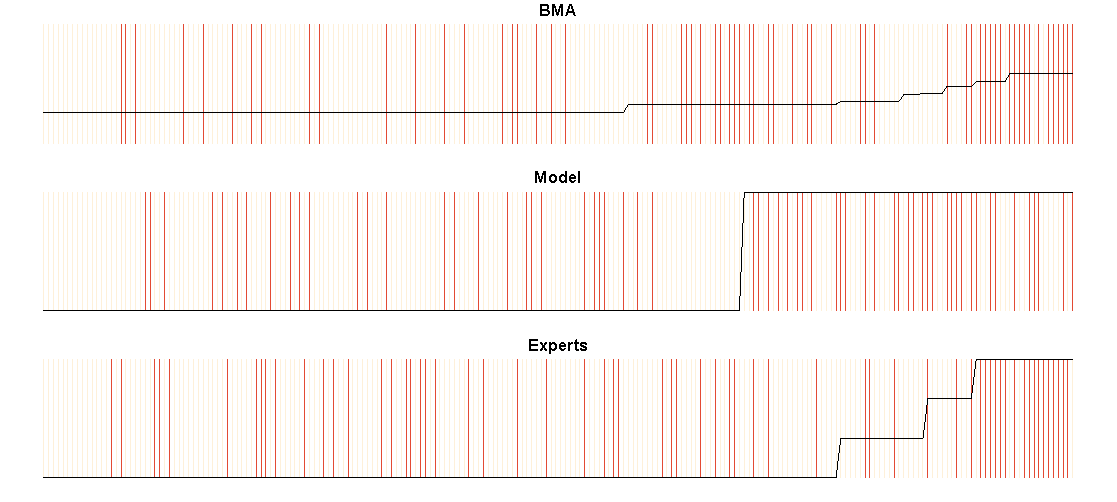
\includegraphics[width=6.5 in]{SCPlot.PDF}
%\end{center}
%\end{figure}

There is a long-standing debate in may circles of the relative
strengths and weaknesses of statistical models and subject experts for
making predictions \citep[e.g.,][]{Ascher:1979}.  Models that use
quantifiable measurements and widely available (if sometimes crude)
data to make predictions can make egregious errors in particular
cases.  Some cases may be decided by forces invisible to the
statistical model but obvious to experts familiar with the case.
Subject experts, on the other hand, can become too focused on minutia
and miss larger (if more subtle) trends in the data easily recognized
by more advanced methodologies.  However, the EBMA technique offers a
theoretically motivated way to combine the strengths of both methods,
while smoothing over their relative weaknesses, to make more accurate
predictions.

\section{Proposed research and timeline}

Thus far, we have extended prior research to make EBMA applicable to
binary and continuous outcomes in political science.  As the above
examples demonstrate, the method already increases the accuracy of
predictions.  However, we propose to expand this research in four
ways.

\textbf{Fully Bayesian estimation:} MCMC estimation of EBMA models can
more efficiently handle a wider variety of predictive distributions
\citep{Vrugt:2008}.  Standard Bayesian methods, such as data
augmentation, will allow us to build a set of statistical results and
computer algorithms appropriate for an array of assumed outcome
distributions.  Specifically, we plan to conduct basic research to
develop a class of models and MCMC samplers to handle continuos,
censored-continuous, binary, and event count data.\footnote{Moreover,
  as the number of parameters is relatively moderate, Bayesian
  algorithms also promise to provide fast results while eliminating
  concerns about false convergence to local maxima that can occur when
  using EM methods.}

\textbf{Alternative model weights}: Currently, model weights are
calculated based solely on the model's deterministic forecast (i.e.,
their point predictions). Even for continuous data, the current EBMA
model assumes that within-forecast variances ($\sigma^2$) is constant.
In other words, model weights do not reflect the uncertainty
associated with each model's predictions.  Applying both Bayesian and
bootstrap methods, we intend to incorporate the entire predictive PDFs
of component forecasts so that model weights reflect not only
components' accuracy, but also their precision.  Poorly calibrated
models should be penalized and receive less posterior weight.

A related issue is that EBMA makes no adjustment for model complexity.
That is, model weights are based solely on the components'
goodness-of-fit with no effort to adjust for their generalizability.
This can lead to excessive
weighting of complex and over-fit models. Since component forecasts
may be agent-based models, stochastic simulations, multi-level models,
and the like, it is necessary to go beyond merely penalizing for the
number of parameters (e.g., AIC). Complexity measures must take into
account functional form and other concerns. As part of continued
research, we plan to incorporate several proposed methods for
penalizing complexity into the EBMA method \citep[c.f.,][]{Pitt:2002a,
  Pitt:2002b, Spiegelhalter:2002}, implement
these priors in our software, and test them against existing vague
priors using both simulated and real-world data.

\textbf{Software:} We will develop open-source software that will be
publicly available.  Specifically, we will produce an R package that
implements both the binary outcome version we have already developed
and the additional extensions just discussed.  Moreover, the package
will provide a more flexible interface for users interested in
ensemble forecasting outside of the weather prediction community than
is currently available.  

Our specific goals for the software package include: S4 compliance,
computationally efficient internal functions written either in C or
Java, handling of multiple outcome distributional assumptions and
priors with a small set of user functions, Gaussian copula techniques
for handling missing data \citep{Hoff:2007}, customizable data
visualizations to facilitate EBMA and component model comparisons,
exemplar datasets and vignettes based on real-world
applications of the method to the social and physical sciences, and
built-in convergence diagnostics for all Bayesian methods compatible
with the `coda' and `boa' packages in R.  At the completion of the
project, we will submit and article to the \textit{Journal of
  Statistical Software} explaining both the technical details of the
package and providing tutorials explaining its available features.

\textbf{Dissemination of findings}: Beyond providing the software and
its attendant documentation, we will disseminate the results of our
research in three ways.  First, we will submit articles explaining the
mathematical and technical details of EBMA to journals in political
methodology, economics, and applied statistics.  Second, we plan to
develop and publish at least two extended applications of the method
to topics in political science.  Our particular focus here will be:
(1) improved forecasting of international crisis events; (2) election
forecasting with the aim of collaborating with other scholars to
generate ensemble predictions for the 2012 U.S. elections.  Third, we
will offer a workshop on forecasting political outcomes during the
first day of the 2012 meeting of the Political Methods Conference
(already scheduled to be hosted by the UNC and Duke).

\textbf{Project Workplan}:

\noindent \textit{01/2012 -- 06/2010}: In this stage, we will conduct basic
research into MCMC estimation of EBMA and prior structures that
penalize model complexity and ensure that posterior estimates reflect
uncertainty in component forecasts.

\noindent \textit{07/2012 -- 06/2013}: In this stage, we will develop,
test, and document the software. This will also involve gathering
exemplar forecasting datasets for inclusion in package vignettes.
These examples will be the basis for subsequent applied research and
publication.

\noindent \textit{07/2013 -- 12/2013}: This stage will focus on: (1)
preparing software and documentation for public dissemination,
improving user interfaces, and increasing the computational efficiency
of internal functions, and (2) revision and submission of results for
publication.



\section{Results from Prior NSF Support}

\subsection{NSF Grants Received by Michael D. Ward During Previous 5 Years}

\begin{enumerate}

\item 0827016 (\$749,970; PI's sub \$150,000) AOC: The Dynamics of
  Secessionist Regions: Eurasian Unrecognized Quasi-States after
  Kosovo's Independence 10/01/2008--09/30/2011

\item 0631531 (\$400,000) Longitudinal Network Modeling of
  International Relations Data 11/15/2006--10/31/2009

\item 0433927 (\$650,000; PI's sub \$150,000) The Dynamics of Civil
  War Outcomes: Bosnia and the North Caucasus 10/01/2004--09/30/2008

\item 0417559 (\$150,000) Network Modeling of International Peace and
  Trade Data 10/01/2004--09/30/2006

\item 0631531 () Longitudinal Network Modeling of International Relations Data  
\end{enumerate}  Only one of these grants is still open (\# 1), but these funds have
only recently (Spring 2011) been transferred to Duke University. The
most relevant grant is \# 5, which is discussed below. \vspace{.1in}

\textit{Summary of Findings:} One of our primary findings is that
standard hazard regression methods for longitudinal relational data,
using variants of proportional hazards models, are unable to properly
account for temporal or relational dependence in IR data. We have
explored several approaches to modeling the longitudinal dependencies.
One models temporal correlations directly as a network.  A second uses
the temporal evolution of the latent network as a means of imparting
dynamic structure into the estimation of the network parameters.  A
final approach, which we are completing now, involves modeling a
separate time-series regression for each pair of countries, but using
a special array-variate hierarchical model to allow for similarity in
trade patterns across groups of countries. We show that the
regularized estimates from this hierarchical model outperform existing
methods in out-of-sample prediction of longitudinal trade data.

\textit{Broader Impacts:} We have presented the research at a number
of conferences and in-departmental seminars in the fields of
statistics, biostatistics, political science, and geography. We have
created the first installment of a series of open-source software
packages for the analysis of relational data. These packages are
widely used in the social science community conducting network
analyses. Finally, we constructed a database of trade and conflict
that can be accessed by our software.

Within the first year we completed the following: (1) trained a
graduate student in the analysis of longitudinal relational data; (2)
constructed and analyzed databases on longitudinal international
relations data (including data on conflicts, trade, currency exchange,
membership in IGOs); (3) developed new statistical methodologies for
multivariate and longitudinal data; (4) conducted basic research in
the area of multivariate statistical models, including methods related
to copula modeling and reduced-rank matrix models; (5) conducted basic
research into the analysis of array data, such as longitudinal trade
data, using random-effects versions of multiway array methods such as
PARAFAC, and developed an extension of the multivariate and
matrix-variate normal distribution appropriate for modeling multiway
array data.

Finally, two students learned how to gather and organize data, write
technical documents, and perform independent research. Both students
completed their Ph.D. in the summer of 2010. One student (John
Ahlquist) received two national awards for his dissertation.

\textit{Publications Resulting from Award:}

\begin{list}{\labelitemi}{\leftmargin=1em} \small
\item Ward, Michael D., Randolph M. Siverson, and Xun Cao. 2007. ``Disputes, Democracies, and Dependencies: A Re-examination of the
  Kantian Peace''. \newblock {\textit{American Journal of Political
    Science}} 51(3):583-601.

\item Ward, Michael D. and Peter D. Hoff. 2008. Analyzing
  Dependencies in Geo-Politics and Geo-Economics.  \newblock In \textit{ Contributions to
    Conflict Management, Peace Economics, and Development, Volume 6,
    War, Peace and Security}, ed. Jacques Fontanel and Manas Chatterji. Bingley, UK: Emerald Publishing, pp. 133-160. % not sure this is correct yet

\item Krivitsky, Pavel, Mark Handcock, Adrian Raftery and Peter Hoff. 2009. ``Representing Degree Distributions, Homophily and Clustering in
  Social Networks with Latent Cluster Models". \newblock{\textit{Social Networks}} 31(3):204-213.

\item  Hoff, Peter. 2008. ``Modeling Homophily and Stochastic Equivalence in
  Symmetric Relational Data". \newblock{\textit{Advances in Neural Information %check this one
  Processing Systems}} 20: 667-674.

\item Hoff, Peter. 2009. ``Simulation of the Matrix Bingham-von-Mises-Fisher
  Distribution, With Applications to Multivariate and Relational
  Data". \newblock{\textit{Journal of Computational and Graphical Statistics}} 18(2):438--456.

\item Hoff, Peter. 2009. ``A hierarchical eigenmodel for pooled covariance
  estimation". \newblock{\textit{Journal of the Royal Statistical Society: Series
  B (Statistical Methodology)}} 71(5):971--992.
  
\item Ward, Michael D. 2010. Statistical Analysis of
  International Interdependencies. In \newblock {\textit{The International  %check this one
    Studies Encyclopedic Compendium: Scientific Studies of
    International Processes, Volume 10}}, ed. Paul F. Diehl and
  James D. Morrow, pp. 6615-6628.
  
\item Bakke, Kristin M., Xun Cao, John O'Loughlin and Michael D. Ward. 2009. ``Social Distance in Bosnia and the North Caucasus Region
  of Russia: Inter- and intra-ethnic attitudes and identities''. \newblock {\textit{Nations and Nationalism}} 15(2):227-253.

\item Hoff, Peter. 2011. ``Hierarchical multilinear models for multiway
  data". \newblock{\textit{Computational Statistics and Data Analysis}} 55(1):530--543.

\item Hoff, Peter and Xiaoyue Niu. 2010. ``A covariance regression model". \newblock{\textit{Statistica Sinica}} Submitted.


\item  Ahlquist, John S. 2008. ``Building and Using Strategic Capacity: Labor Union Confederations and Economic Policy". Thesis. Published. %check this
Bibliography: Doctoral Dissertation, University of Washington.

\item  Raftery, Adrian E. and Michael D. Ward. 2010. \newblock{\textit{Statistical Methodology: Special Issue on Statistical Methods for the Social Sciences}}. %check this
Elsevier. Volume 8.
\end{list}

 \subsection{NSF Grants Received by Jacob M. Montgomery}
\begin{enumerate}
\item SES-1023762  (\$12,000) Doctoral Dissertation Research in Political Science: The Causes, Consequences, and Measurement of Perceived Political Control, 09/2010-08/2011.    
\end{enumerate}

\textit{Summary of Findings:} I developed, evaluated, and validated a
measure of perceived political control. I show that the scale is
distinct from extant measures, and has superior explanatory power for
predicting important behaviors in the future. In work currently
underway, I show that actively supporting a winning candidate plays a
causal role in shaping these control beliefs.

\textit{Broader Impacts:}I have presented the research at a
conference.  In addition, I developed an online platform for applying
computer-based psychological testing techniques for more efficient
administration of large scale in online surveys to be released for
public use.

\textit{Publications:}

\begin{list}{\labelitemi}{\leftmargin=1em} \small
\item Jacob M. Montgomery, ``An Evolutionary Theory of Democracy:
  Dynamic Evolutionary Models of American Party Competition with an
  Empirical Application to the Case of Abortion Policy from
  1972-2010'', Doctoral Dissertation, Duke University, Sept (2010).
\end{list}


\newpage
\setcounter{page}{1}

 \bibliographystyle{apsr}
\bibliography{Flo_Bib_PA}
%\bibliography{/Users/mw160/Documents/BIBTEXFILES/predictionrefs/predictions2,/Users/mw160/Documents/BIBTEXFILES/2009mdwbib}}

\newpage
\setcounter{page}{1}


\section*{Michael D. Ward}
\subsection*{Professional Preparation}
\begin{itemize}
\item[]B.A. (Honors), Indiana University, 1970. 
\item[]Ph. D., Political Science, Northwestern University, 1977. 
\item[]Gordon Scott Fulcher Post Doctoral Research Associate \& Visiting Assistant Professor, Department of Political Science, Northwestern University, 1977-1980.
\end{itemize}
\subsection*{Appointments}
\begin{itemize}
\item[] Professor of Political Science, Duke University, 2009--present.
\item[] Professor of Political Science, University of Washington, 1997--2009.
\item[] Chaire Municipale \& Professeur, Facult\'{e} des Sciences \'{E}conomiques, Universit\'{e} Pierre Mend\`{e}s France, Grenoble, France, 2000-2005.
\item[] Professeur Invit\'{e}e et Emerit\'{e}, Facult\'{e} des Sciences \'{E}conomiques, Universit\'{e} Pierre Mend\`{e}s France, Grenoble, France, 1990-1991.
\item[] Professor of Political Science, University of Colorado, 1982-1998.
\item[] Research Scientist, Wissenschaftszentrum Berlin, International Institute for Comparative Social Research, 1980-1982.

\item[] Gordon Scott Fulcher Post Doctoral Research Associate \& Visiting Assistant Professor, Department of Political Science, Northwestern University, 1977-1980.
\end{itemize}
\subsection*{Publications}
\subsubsection*{Related to Proposed Activities}
\begin{itemize}

\item[1] Weidmann, Nils B. and Michael D. Ward. 2010. ``Predicting Conflict in Space and Time''. \newblock {\textit{Journal of Conflict Resolution}} 54(6): 883-910.

\item[2] Ward, Michael D., Brian D. Greenhill and Kristin M. Bakke. 2010. ``The Perils of Policy by P-Value: Predicting Civil Conflicts''. \newblock {\textit{Journal of Peace Research}} 48(4):3673-375. (Winner of best article in journal during 2010).

\item[3] Ward, Michael D. and Kristian Skrede Gleditsch. 2008. \newblock {\textit{Spatial Regression Models}}. Thousand Oaks, California and London: Sage Publishers

\item[4] Greenhill, Brian D., Michael D. Ward and Audrey Sacks. 2011. ``The Separation Plot: A New Visual Method for Evaluating the Predictive Power of Binary Models''. \newblock {\textit{American Journal of Political Science}} in press.

\item[5]
Ward, Michael D. and Kristian Skrede Gleditsch. 2002. ``Location, Location, Location: An MCMC Approach to Modeling the
  Spatial Context of War and Peace''. \newblock {\textit{Political Analysis}} 10(3):244--260.
\end{itemize}

\subsubsection*{Five Other Significant Publications}
\begin{itemize}

\item[1]  Ward, Michael D., Randolph M. Siverson and Xun Cao. 2007. ``Disputes, Democracies, and Dependencies: A Re-examination of the Kantian Peace''. \newblock {\textit{American Journal of Political Science}} 51(3):583-601
   
\item[2]
Ward, Michael D. and Kristian Skrede Gleditsch. 1998. ``Democratizing for Peace''. \newblock {\textit{American Political Science Review}} 92(1):51--61
 
 \item[3] Ward, Michael D. and David~R Davis. 1992. ``Sizing up the Peace Dividend: Economic Growth and Military Spending
  in the {United States}, 1948--1996''. \newblock {\textit{American Political Science Review}} 86(3):748--758.
 
 \item[4]
Mintz, Alex and Michael~D. Ward. 1989. ``The Political Economy of Military Spending in {I}srael''.
\newblock {\textit{American Political Science Review}} 83(2):521--533.

\item[5]
Ward, Michael D. 1984. ``Differential Paths to Parity: A Study of the Contemporary Arms Race''.
\newblock {\textit{American Political Science Review}} 78(2):297--317.

\end{itemize}
\subsection*{Synergistic Activities}
While on the executive council of the Center for Statistics and the
Social Sciences, I helped to develop a university wide curriculum in
applied statistical methods that would be available to social science
departments across the university. We also created new fields of
applied statistics within a total of five departments; our first was
in the department of Political Science. These served to broaden and
deepen training in statistical methods for social science graduate
students at the University of Washington.

I have also organized several conferences aimed at helping scholars in
the social sciences to apply new approaches to the study of social
phenomenon. One of these was a conference at the University of
Washington on Spatial and Network approaches to studying political
phenomenon, which was sponsored in part by the Center for Statistics
and the Social Sciences, but also funded in part by a grant from the
Center for Spatially Informed Social Sciences.

In 2010, I also organized and was the local host for the 2010 Duke
Conference on Networks in Political Science, an international and
multidisciplinary gathering of about 200 scholars and practitioners of
network science.


\subsection*{Collaborators}

\subsubsection*{Collaborators and co-Editors in the past 48 months}
John Ahlquist, Kristin Bakke, Xun Cao, Kristin Gleditsch, Brian
Greenhill, Peter Hoff, Aseem Prakash, Ian Lustic, Nils Metternich,
Clionadh Raleigh, Adrian Raftery, Phil Schrodt, Stephen Shellman,
Randolph Siverson, Katherine Stovall, \& Nils Weidmann.
\subsubsection*{Graduate Advisors and Postdoctoral Sponsors.}
\begin{itemize}
\item[] My advisors: James A. Caporaso (University of Washington),
  Harold Guetzkow (RIP), Karl W. Deutsch (RIP)
\item[] My advisees: John Ahlquist (University of Wisconsin), Xun Cao
  (Penn State University), Brian Greenhill (Dartmouth University),
  Nils Weidmann (Yale University), Umut Aydin (Bo\v{g}azi\c{c}i
  University), Christian Breunig (University of Toronto), Kristian
  Gleditsch (Essex University), David Brown (University of Colorado),
  Michael Shin (UCLA)
\end{itemize}

\newpage


\newpage
\setcounter{page}{1}
\thispagestyle{empty}

\section*{Jacob M. Montgomery}
\subsection*{Professional Preparation}
\begin{itemize}
\item[]B.A. (\textit{Summa Cum Laude}), Wake Forest University, 2002.
\item[]M.S., Statistical Science, Duke University, 2009. 
\item[]Ph. D., Political Science, Duke University, 2011. 
\end{itemize}
\subsection*{Appointments}
\begin{itemize}
\item[] Assistant Professor of Political Science, Washington
  University in St. Louis, 2011--present.
\end{itemize}

\subsection*{Publications}
\subsubsection*{Related to Proposed Activities}
\begin{itemize}
\item[1] Montgomery, Jacob M. and Brendan Nyhan. 2010. ``Bayesian Model Averaging: Theoretical Developments and
Practical Applications''. \newblock {\textit{Political Analysis}} 18(2): 245-270.

\item[2] Montgomery, Jacob M., Alexandra Cooper, Jerome Reiter and Shuo Guan. 2008. ``Non-Response Bias on Dimensions of Political Activity
Amongst Political Elites''. \newblock {\textit{International Journal of Public  Opinion Research}} 20(4): 223-231.
\end{itemize}

\subsubsection*{Other Significant Publications}
\begin{itemize}
\item[1] Aldrich, John H., Jacob M. Montgomery and Wendy Wood. Forthcoming. ``Turnout as a Habit''.\newblock {\textit{Political Behavior}}. 
\newblock \url{http://www.springerlink.com/content/4550l465ux177435/}

\item[2] Montgomery, Jacob M., Kristie Long Foley and Mark Wolfson. 2006. ``Enforcing the Minimum Drinking Age: State, Local, and Agency Characteristics Associated With Compliance Checks and Cops in Shops Programs''. \newblock {\textit{Addiction}} 101(2): 223-231.
\end{itemize}


\subsection*{Synergistic Activities}
From 2008-2010, I helped found and organize a weekly methods

workshop involving faculty and graduate students at both Duke
University and the University of North Carolina.  

\subsection*{Collaborators}

\subsubsection*{Collaborators and co-Editors in the past 48 months}
John H. Aldrich (Duke), Alexandra Cooper (Duke), Christophe DeSante
(Duke), Melanie Freeze (Duke), Shuo Guan, David Neal (University of Southern
California -- Psychology), Brendan Nyhan (Dartmouth), Jerome Reiter
(Duke -- Statistical Science), David Sparks (Duke), Wendy Wood
(University of Southern California -- Psychology).

\subsubsection*{Graduate Advisors and Postdoctoral Sponsors.}
\begin{itemize}
\item[] Ph.D. Dissertation Advisors: John H. Aldrich (Duke), Nancy Burns
  (University of Michigan), Michael C. Munger (Duke), David Rohde (Duke)
\item[] M.S. Thesis Advisors: Jerome Reiter (Duke -- Statistical Science), David Dunson
  (Duke -- Statistical Science)
\end{itemize}

\newpage
\setcounter{page}{1}
\thispagestyle{empty}

\section*{Data Management Plan}

\noindent Data and programs from this research will be deposited in a Dataverse archive at \url{thedata.org} within 12 months of the end of the project.

\newpage
\setcounter{page}{1}
\thispagestyle{empty}

\section*{Budget Justification (DUKE)}

The PI, Michael Ward, is budgeted for 0.5 months in each year.  The
faculty benefit rate for Ward is XX\%.   

The PIs ask for \%XX,XXX to cover the cost of a graduate assistant at
Duke University budgeted to work at 50\% effort for one year (June,
2012 - May, 2013).  The graduate student benefit rate is XX.X\%.  The
combined cost for graduate student assistance will be \$XX,XXX.

The PIs ask for \$2,500 for travel.  This money is expected to cover 1
trip for in-person collaborative research in St. Louis, MO.  In addition,
the PI and one graduate student will attend the yearly Political
Methodology Conference.

Finally, Duke University's current indirect cost rate with DHHS is 6X.X\%.



\newpage
\setcounter{page}{1}
\thispagestyle{empty}

\section*{Budget Justification (Washington University in St. Louis)}

The CO-PI, Jacob M. Montgomery, is budgeted for 1 months in each year.  The
faculty benefit rate for Montgomery is XX\%.   The combined cost will
be \$25,000.

The PIs ask for \%XX,XXX to cover the cost of a graduate assistant at
Washington University in St. Louis budgeted to work at 50\% effort for one year
(June, 2012 - May, 2013).  The graduate student benefit rate is
XX.X\%.  The combined cost for graduate student assistance will be
\$XX,XXX.

The PIs ask for \$2,500 for travel.  This money is expected to cover 2
trips for in-person collaborative research in Durham, NC.  In
addition, Montgomery will attend the yearly Political Methodology
Conference.

Finally, Washington University's current indirect cost rate with DHHS is 5X.X\%.

\newpage
\setcounter{page}{1}
\section*{TODO}

\begin{enumerate}
\item Florian to review references to ensure that they include: article title,
  journal title, volume number, page numbers, authors, and year of
  publication.  
\item Budget (one for each school)
\item Budget justification (One for each school)
\item Facilities, Equipment and Other Resources (one for each school)
\item Make all of this conform to the ``collaborative proposals''
  guidelines reproduced belo.
\item Get the Fastlane ``cover sheet'' filled out correctly (and identically in
  both locations).
\end{enumerate}



4. Collaborative Proposals  (pg. II-23

A collaborative proposal is one in which investigators from two or
more organizations wish to collaborate on a unified research project.
Collaborative proposals may be submitted to NSF in one of two methods:
as a single proposal, in which a single award is being requested (with
subawards administered by the lead organization); or by simultaneous
submission of proposals from different organizations, with each
organization requesting a separate award.  In either case, the lead
organization’s proposal must contain all of the requisite sections as
a single package to be provided to reviewers (that will happen
automatically when procedures below are followed).  All collaborative
proposals must clearly describe the roles to be played by the other
organizations, specify the managerial arrangements, and explain the
advantages of the multi-organizational effort within the Project
Description.  PIs are strongly encouraged to contact the cognizant NSF
Program Officer prior to submission of a collaborative proposal.

a. Submission of a collaborative proposal from one organization The
single proposal method allows investigators from two or more
organizations who have developed an integrated research project to
submit a single, focused proposal.  A single investigator bears
primary responsibility for the administration of the grant and
discussions with NSF, and, at the discretion of the organizations
involved, investigators from any of the participating organizations
may be designated as co-PIs.  Please note, however, that if awarded, a
single award would be made to the submitting organization, with any
collaborators listed as subawards.

If a proposed subaward includes funding to support postdoctoral
researchers, the mentoring activities to be provided for such
individuals must be incorporated in the supplemental mentoring plan
outlined in GPG Chapter II.C.2j.

By submission of the proposal, the organization has determined that
the proposed activity is administratively manageable.  NSF may request
a revised proposal, however, if it considers that the project is so
complex that it will be too difficult to review or administer as
presented.  (See GPG Chapter II.C.2g.(vi)(e) for additional
instructions on preparation of this type of proposal.)

 b. Submission of a collaborative proposal from multiple organizations

In many instances, simultaneous submission of proposals that contain
the same Project Description from each organization might be
appropriate.  For these proposals, the project title must begin with
the words ``Collaborative Research:''.  The lead organization's
submission will include a Cover Sheet, Project Summary, Project
Description, References Cited, Biographical Sketches, Budgets and
Budget Justification, Current and Pending support, and Facilities,
Equipment and Other Resources for their organization.  If applicable,
the lead organization’s submission also must include a supplemental
mentoring plan that must not exceed one page, and that addresses the
mentoring activities to be provided for all postdoctoral researchers
supported under the entire collaborative project.  See GPG Chapter
II.C.2.j for additional guidance on mentoring and data management plan
requirements for collaborative proposals.  Non-lead organization
submissions will include all of the above for their organization
except the project summary, project description, and references cited
which are the same for all collaborating organizations.  FastLane will
combine the proposal submission for printing or electronic viewing.

To submit the collaborative proposal, the following process must be
completed: 

(i) Each non-lead organization must assign their proposal a proposal
PIN.  This proposal PIN and the temporary proposal ID generated by
FastLane when the non-lead proposal is created must be provided to the
lead organization before the lead organization submits its proposal to
NSF. 

(ii) The lead organization must then enter each non-lead
organization(s) proposal PIN and temporary proposal ID into the
FastLane lead proposal by using the "Link Collaborative Proposals"
option found on the FastLane "Form Preparation" screen.  Given that
such separately submitted proposals constitute a “single” proposal
submission to NSF, it is imperative that the proposals be submitted
within a reasonable timeframe to one another.  

(iii) All components of the collaborative proposal must meet any
established deadline, and, failure to do so may result in the entire
collaborative proposal being returned without review.




\end{document}
\bye
